\documentclass[11pt,a4paper]{article}
\usepackage[hyperref]{acl}

\usepackage{times}
\usepackage{latexsym}
\usepackage{microtype}
\usepackage{placeins}

\usepackage{graphicx}
\usepackage{booktabs}
\usepackage{multirow}
\usepackage{url}

\usepackage{tikz}
\usetikzlibrary{arrows.meta,positioning,fit,shapes.geometric,shapes.misc}

\title{Legitimizing Facial Recognition}

\author{
  Lakshya Jain \\
  {\tt lakshyajain}
  \And
  Rishita Valluru \\
  {\tt rishitavalluru}
}

\begin{document}
\maketitle

\begin{abstract}
Facial recognition technologies are widely deployed across commercial and public-sector contexts, even as they remain ethically and politically contested. Vendors respond to these tensions by constructing public-facing narratives that seek to normalize adoption and establish legitimacy. This paper presents a reproducible, longitudinal analysis of how facial-recognition vendors articulate legitimacy through corporate website discourse.

Using archived web snapshots from the Internet Archive, we construct a multi-decade corpus of vendor-facing text and apply a domain-specific cleaning and filtering pipeline to retain facial-recognition–relevant content. We use \textsc{BERTopic} to identify recurring thematic structures in heterogeneous corporate language and introduce transparent, dictionary-based metrics to quantify ethical, surveillance, and market-oriented legitimacy framing at the company and company-year levels.

Our results show that vendor discourse is organized around distinct and interpretable topics with limited redundancy, despite substantial textual heterogeneity. Temporal analysis highlights the concentration of discourse in the 2010s and 2020s and reveals systematic variation in framing strategies across vendors. Together, these methods provide scalable quantitative structure alongside traceable qualitative evidence for analyzing corporate legitimacy in contested sociotechnical systems.
\end{abstract}

\section{Introduction}
Facial recognition and adjacent biometric technologies have expanded rapidly across commercial and public-sector settings. At the same time, these technologies raise persistent questions about privacy, fairness, accountability, and governance. In such contexts, firms do not merely ship products; they also communicate narratives that aim to normalize adoption, mitigate perceived risks, and justify legitimacy to customers, regulators, and the public. Corporate websites are a primary channel for this communication, but they are inherently dynamic: product positioning, compliance claims, and ethical language evolve in response to shifting market incentives, regulation, and public scrutiny.

This paper reports a hybrid (academic framing + technical transparency) study that analyzes longitudinal corporate language associated with facial recognition vendors. We operationalize legitimacy framing as recurring patterns of public-facing textual claims, and we develop a reproducible pipeline that enables large-scale analysis across vendors and time. Our approach uses archived web snapshots, domain-specific text extraction and filtering, BERTopic-based topic modeling, and keyword-dictionary framing metrics to identify themes and quantify the relative emphasis on ethical, surveillance, and market legitimacy appeals.

\paragraph{Contributions.}
This work makes four contributions:
\begin{enumerate}
\item A reproducible archival data collection and cleaning pipeline for vendor website snapshots, including relevance filtering and deduplication.
\item A BERTopic-based topic modeling workflow optimized for improved topic granularity and interpretability.
\item A transparent framing analysis that produces company-level and company-year legitimacy framing scores (ethical, surveillance, market) based on explicit keyword dictionaries.
\item Company-level profiles combining dominant topics, topic descriptions, framing scores, timelines, and representative excerpts to support mixed-method interpretation.
\end{enumerate}

\paragraph{Research Questions.}
Guided by prior work on corporate legitimacy and contested technologies, this study addresses the following research questions:
\begin{enumerate}
\item What dominant discursive themes characterize how facial-recognition vendors present and justify their technologies on corporate websites?
\item How do these themes vary across time, particularly as the volume of corporate web content increases in the 2010s and 2020s?
\item How do vendors differ in their relative emphasis on ethical, surveillance, and market-oriented legitimacy framing?
\end{enumerate}

\section{Related Work}
This section situates the project at the intersection of (i) corporate legitimacy and self-presentation in contested markets, (ii) computational social science methods using web archives, and (iii) topic modeling for thematic discovery and temporal analysis in large text corpora. We emphasize methodological alignment with mixed-methods research: automated extraction and modeling provide scalable structure, while outputs such as representative documents and company profiles support interpretive follow-up.

\section{Data Collection}
\subsection{Vendor Identification}
We construct a vendor universe grounded in facial-recognition-related actors. The vendor list is used as the starting point for web snapshot retrieval and subsequent downstream analysis. The vendor universe may combine multiple sources (e.g., performance evaluation vendor lists and curated compilations), and all collection steps are designed to remain reproducible.

\subsection{Wayback Snapshot Retrieval}
We use the Internet Archive's Wayback Machine to retrieve historical snapshots of vendor websites. The archive provides access to time-indexed captures of web pages, enabling longitudinal analysis of corporate language even when current websites have changed substantially.

\paragraph{Snapshot Scope}
Before downloading archived HTML content, we first examined the temporal availability of Wayback snapshots across the set of facial-recognition vendors. For each company, we recorded the first and last archived website snapshots and used this range as an indicator of when the vendor maintained a public-facing web presence. We then aggregated these ranges to estimate how many vendors were observable in the archive at different points in time.

This scoping step showed sparse coverage before the late 1990s, gradual growth through the 2000s, and a sharp increase beginning around 2010. Vendor presence reaches its highest levels in the early 2020s, with a small decline in the most recent years that likely reflects incomplete archival capture rather than changes in the industry itself. These patterns were used to guide sampling decisions and to set expectations about temporal imbalance in the downstream corpus; substantive analysis of vendor discourse is conducted only after HTML cleaning and is presented in later sections.

\paragraph{Snapshot Strategy.}
Our collection strategy retrieves archived HTML pages for vendors across decades. For each vendor and time range, we retrieve relevant HTML pages and organize them into a structured directory layout by vendor and decade, preserving the mapping between each text document and its archival path. This enables both aggregate analysis (topic distributions across the corpus) and stratified analysis (e.g., per decade, per vendor).

\paragraph{Ethical and Operational Constraints.}
To reduce load on third-party services and avoid unnecessary repeated requests, collection is implemented with throttling and retries, and downstream processing is designed to operate on locally stored snapshots. This design supports research reliability and operational safety.

\section{Data Cleaning and Filtering}
To support reliable topic modeling and framing analysis, we apply a multi-stage cleaning pipeline to convert archived HTML snapshots into cleaned text documents. The goal is to remove boilerplate and interface artifacts (e.g., navigation menus, cookie banners) and retain content-bearing text relevant to facial recognition and adjacent identity technologies.

\subsection{HTML Cleaning}
We parse HTML with a structured parser and remove non-content elements (e.g., scripts/styles, navigation, headers/footers, forms). We also remove common cookie and consent banners using class/id pattern matching, and we whitelist content-bearing tags (e.g., \texttt{article}, \texttt{main}, headings, paragraphs, list items). We then normalize whitespace and fix encoding artifacts.

\subsection{Language Filtering}
We restrict the corpus to English-language documents to maintain consistency for topic modeling and to reduce noise introduced by multilingual pages in an archive-driven dataset. Language detection is applied on a short snippet of each cleaned document.

\subsection{Domain Relevance Filtering}
Because vendor websites can contain generic corporate content, we apply a facial-recognition relevance filter based on a curated list of domain keywords (e.g., \textit{facial recognition}, \textit{liveness detection}, \textit{identity verification}, \textit{access control}, \textit{video surveillance}, \textit{privacy}, \textit{responsible AI}). Documents not containing any relevance keywords are removed.

\subsection{Length Thresholding and Deduplication}
We remove very short pages that are unlikely to contain meaningful content. We also remove duplicates across vendor, decade, and cleaned text to account for repeated archival captures, template pages, and replicated boilerplate.

\begin{table}[t]
\centering
\small
\begin{tabular}{lrr}
\toprule
\textbf{Decade} & \textbf{Documents} & \textbf{Percentage} \\
\midrule
1990s & 3    & 0.03\% \\
2000s & 342  & 3.42\% \\
2010s & 1857 & 18.58\% \\
2020s & 7792 & 77.97\% \\
\midrule
\textbf{Total} & 9994 & 100.00\% \\
\bottomrule
\end{tabular}
\caption{Distribution of cleaned, retained documents by decade (computed from the merged cleaned corpus).}
\label{tab:decade_distribution}
\end{table}

\section{Topic Modeling Methodology}
\subsection{BERTopic Overview}
We use \textsc{BERTopic} to discover coherent themes in the cleaned corpus. BERTopic combines transformer-based embeddings with clustering to produce topics represented by salient words and representative documents. This approach is suitable for heterogeneous corporate text because it can capture semantic similarity beyond surface word overlap while still returning interpretable topic descriptors.

\subsection{Model Components and Settings}
We configure BERTopic with: (i) a sentence-transformer embedding model, (ii) \textsc{UMAP} for dimensionality reduction, (iii) \textsc{HDBSCAN} for density-based clustering, and (iv) a count vectorizer for topic-word representations. To improve granularity and avoid a small number of dominant topics, we use more sensitive clustering settings and fix a target number of topics (e.g., 40) for interpretability.

\subsection{Quality Controls and Interpretability}
We assess topic coherence and separation using:
\begin{enumerate}
\item Intertopic distance visualization for global structure,
\item Hierarchical clustering for topic relationships,
\item Similarity matrices for pairwise topic proximity,
\item Term-rank curves to evaluate topic-word score decline.
\end{enumerate}
Additionally, we compute topic summaries (top words, representative documents, top associated companies) to support qualitative interpretation and reporting.

\paragraph{Interpretive role of topics.}
In this study, topics are not treated as fixed ontological categories or as ground-truth representations of firm behavior. Instead, they function as empirical traces of recurring discursive patterns in corporate self-presentation. Topics provide an analytical scaffold that supports (i) summarization of dominant narratives, (ii) comparison across time and vendors, and (iii) contextualization of framing scores and company-level profiles. All substantive claims are therefore grounded in topic summaries and representative documents rather than topic labels alone.

\begin{figure}[t]
\centering
\includegraphics[width=\linewidth]{figs/topic_term_rank.png}
\caption{Term score decline per topic. Steeper declines indicate coherent topic-word distributions, while flatter curves suggest diffuse or generic topics.}
\label{fig:term_rank_main}
\end{figure}

\begin{figure*}[t]
\centering
\resizebox{\textwidth}{!}{%
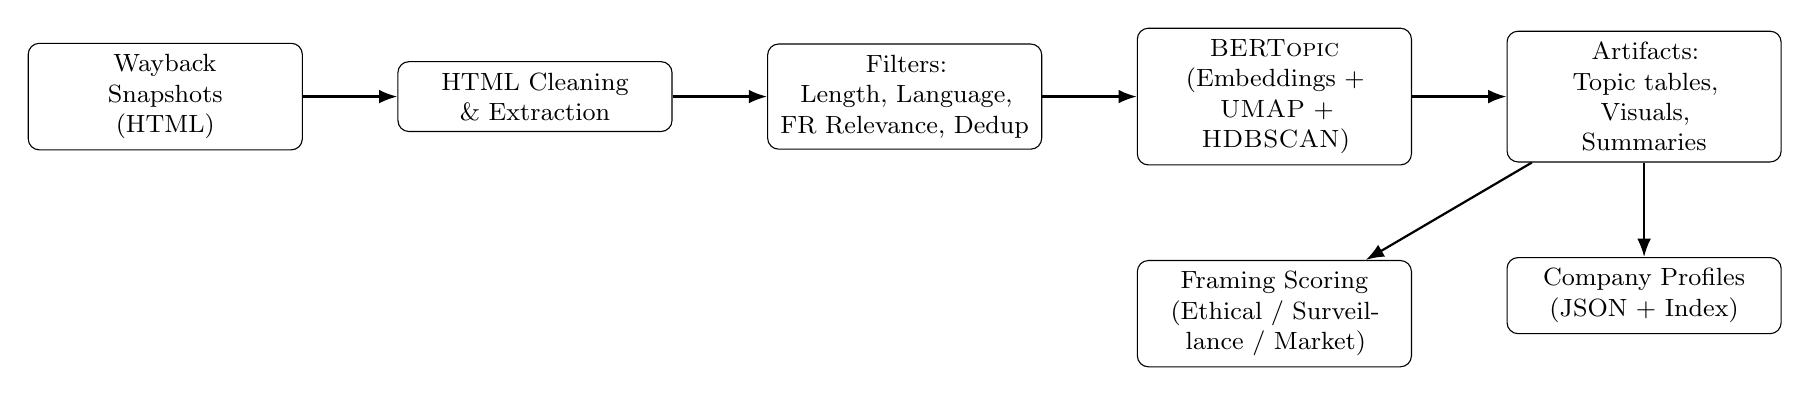
\begin{tikzpicture}[
    node distance=10mm,
    box/.style={
        draw,
        rounded corners,
        align=center,
        inner sep=4pt,
        font=\small,
        text width=3.2cm
    },
    line/.style={-Latex, thick}
]

\node[box] (crawl) {Wayback\\Snapshots\\(HTML)};
\node[box, right=12mm of crawl] (clean) {HTML Cleaning\\\& Extraction};
\node[box, right=12mm of clean] (filter) {Filters:\\Length, Language,\\FR Relevance, Dedup};
\node[box, right=12mm of filter] (topic) {%
\textsc{BERTopic}\\
(Embeddings +\\ \textsc{UMAP} + \textsc{HDBSCAN})
};
\node[box, right=12mm of topic] (outputs) {Artifacts:\\Topic tables,\\Visuals,\\Summaries};

\node[box, below=12mm of topic] (frame) {Framing Scoring\\(Ethical / Surveillance / Market)};
\node[box, below=12mm of outputs] (profiles) {Company Profiles\\(JSON + Index)};

\draw[line] (crawl) -- (clean);
\draw[line] (clean) -- (filter);
\draw[line] (filter) -- (topic);
\draw[line] (topic) -- (outputs);
\draw[line] (outputs) -- (frame);
\draw[line] (outputs) -- (profiles);

\end{tikzpicture}%
}
\caption{Pipeline overview: archival collection, cleaning and filtering, topic modeling, framing analysis, and per-company profiling.}
\label{fig:pipeline_overview}
\end{figure*}

\section{Temporal Topic Analysis}
We augment each document with a timestamp derived from the archival path. This enables frequency-based comparisons across time (e.g., by decade) and allows visualization of topic prevalence over time.

\paragraph{Decade-Level Trends.}
Table~\ref{tab:decade_distribution} shows that the majority of retained documents originate from the 2020s. This distribution is consistent with increased archival coverage and expanded vendor web presence during recent years, and it informs how we interpret temporal dynamics (e.g., sparse coverage prior to 2000).

\paragraph{Topic Prevalence Over Time.}
We compute topic frequencies across timestamps and decades, generating summaries such as \texttt{topic\_over\_time.csv} and \texttt{topics\_per\_decade.csv}. These artifacts support claims about whether particular legitimacy narratives persist, emerge, or shift in emphasis over time.

Importantly, temporal comparisons are interpreted in light of uneven archival density. Rather than assuming uniform historical coverage, we treat data volume itself as informative: the expansion of archived corporate web content in the 2010s and 2020s reflects both technological diffusion and increased regulatory and public scrutiny. As a result, temporal patterns are analyzed as shifts in observed discourse rather than definitive measures of historical prevalence.

\section{Corporate Framing Analysis}
\subsection{Framing Categories}
We operationalize three legitimacy framing categories:
\begin{enumerate}
\item \textbf{Ethical framing:} language emphasizing privacy, fairness, accountability, transparency, and regulatory alignment.
\item \textbf{Surveillance framing:} language emphasizing public safety, threat detection, law enforcement, and monitoring capabilities.
\item \textbf{Market framing:} language emphasizing enterprise readiness, scalability, compliance readiness, onboarding efficiency, and commercial trust, often positioning facial recognition as a routine infrastructure component rather than a contested technology.
\end{enumerate}

\subsection{Keyword Dictionary Construction}
Each framing category is represented by an explicit keyword list that can be audited and modified. Keywords were selected to capture common corporate legitimacy signals found in identity and biometric markets. While dictionary methods cannot capture all nuance, they provide transparent, reproducible signals that can be compared across companies and time.

\subsection{Scoring Method}
For each unit of analysis (company, or company-year), we count keyword occurrences per category across the relevant document set. We then normalize by the total keyword hits across all categories to produce proportions in $[0,1]$ for ethical, surveillance, and market framing. We additionally store the number of documents used in the aggregation.

\begin{table}[t]
\centering
\small
\begin{tabular}{p{0.26\linewidth}p{0.66\linewidth}}
\toprule
\textbf{Category} & \textbf{Illustrative keyword examples} \\
\midrule
Ethical &
responsible AI; trustworthy AI; fairness; transparency; accountability; privacy by design; data protection; GDPR; compliance; regulation \\
Surveillance &
public safety; threat detection; situational awareness; law enforcement; crime prevention; forensic; suspect identification; watchlist; border control \\
Market &
enterprise-grade; compliance-ready; scalable; high availability; frictionless onboarding; digital trust; identity assurance; KYC; AML \\
\bottomrule
\end{tabular}
\caption{Framing categories and representative keyword examples used for dictionary-based scoring.}
\label{tab:framing_keywords}
\end{table}

\section{Company-Level Profiles}
To support interpretability and mixed-method follow-up, we generate per-company profiles that combine: (i) dominant topics by document count, (ii) short topic descriptions based on top words, (iii) framing scores, (iv) a simple temporal timeline of topic counts, and (v) sample document excerpts. Profiles are saved as JSON files with a master index for convenient lookup.

\paragraph{Illustrative Example.}
A profile may show that a given company is dominated by an access-control and identity-management topic, with market framing as the primary legitimacy appeal. Such profiles enable rapid selection of case studies while maintaining transparency about the underlying evidence. By structuring outputs at the company level, the pipeline supports both comparative analysis and deeper qualitative inquiry, aligning computational results with sociological interpretation and course objectives.

\begin{table}[t]
\centering
\small
\begin{tabular}{p{0.30\linewidth}p{0.62\linewidth}}
\toprule
\textbf{Profile field} & \textbf{Description} \\
\midrule
Company & Canonical company identifier (domain) \\
Dominant topics & Top topics by document count (e.g., top 5) \\
Topic descriptions & Short labels derived from top words per topic \\
Framing scores & Ethical / surveillance / market proportions + num\_docs \\
Topic timeline & Topic counts by year (when timestamped) \\
Sample docs & A small set of representative excerpts for reading \\
\bottomrule
\end{tabular}
\caption{Contents of per-company profile JSON artifacts.}
\label{tab:company_profile_fields}
\end{table}

\section{Results}
The results presented above reveal patterned strategies of legitimacy construction that become more interpretable when situated within broader debates about governance, accountability, and contested technological adoption. We report results at three levels: (i) corpus-wide topics, (ii) temporal topic trends, and (iii) framing scores at the company and company-year levels. We also use topic summaries and company profiles to provide interpretive grounding.

\subsection{Corpus-Wide Topic Themes}
Topics serve as a structural layer that organizes the corpus, enables temporal comparison, and contextualizes framing scores, while topic summaries and company profiles provide traceable links to underlying textual evidence. Together, these results reveal recurring legitimacy strategies through which vendors normalize facial-recognition technologies for different audiences.

\subsection{Topic Relationships and Model Diagnostics}
We visualize topic separation and relationships using intertopic distance maps and hierarchical clustering. These diagnostics help assess whether topics reflect meaningful thematic structure or are dominated by generic corporate boilerplate. 

\begin{figure}[t]
\centering
\includegraphics[width=\linewidth]{figs/topics_overview.png}
\caption{Intertopic distance map for the trained \textsc{BERTopic} model. Topics that are spatially separated reflect distinct semantic clusters, while proximity indicates overlapping discursive patterns.}
\label{fig:intertopic_distance_main}
\end{figure}

For example, topics centered on access control and identity management (e.g., Topic~0) tend to co-occur with high market-oriented framing scores, reflecting a discourse that emphasizes enterprise readiness, security infrastructure, and operational efficiency. In contrast, topics associated with surveillance and video analytics (e.g., Topic~2) more frequently align with surveillance framing, highlighting public safety and monitoring narratives. These patterns illustrate how topic structure directly informs interpretation of framing strategies.

\begin{figure}[t]
\centering
\includegraphics[width=\linewidth]{figs/topic_heatmap.png}
\caption{Topic similarity matrix showing pairwise semantic similarity between topics. Lower similarity values indicate limited redundancy and stronger topic separation.}
\label{fig:similarity_matrix_main}
\end{figure}

The similarity matrix indicates that most topic pairs exhibit low to moderate similarity, suggesting limited redundancy across topics. This pattern supports the interpretability of the topic model despite the heterogeneity of corporate web text and indicates that the identified themes capture distinct discursive patterns rather than variations of a single generic narrative. Taken together, these diagnostics indicate that the topic model captures meaningful and distinguishable discursive patterns, providing a reliable foundation for downstream temporal and framing analyses.

\subsection{Temporal Patterns}
We analyze how topic frequencies vary over time and by decade, noting that data density increases sharply in the 2010s and 2020s. This temporal structure is treated as an empirical feature of the archive-derived dataset and explicitly considered when interpreting change.

\subsection{Framing Distributions}
We compute framing scores per company and per company-year to quantify the relative emphasis of ethical, surveillance, and market legitimacy appeals. These scores support comparisons across companies and can be used to select contrasting case studies (e.g., high ethical framing vs.\ high surveillance framing) for deeper qualitative analysis.

Notably, framing distributions vary substantially across vendors. Some firms consistently emphasize ethical and compliance-oriented language, while others prioritize surveillance or market efficiency narratives. These contrasts enable principled selection of divergent case studies and suggest that legitimacy construction in this domain is not uniform but strategically differentiated across organizational contexts. By combining corpus-level modeling with company-specific profiles and representative excerpts, the analysis supports both generalization and interpretive depth.

\section{Discussion}
Our findings suggest that corporate legitimacy construction in this domain often combines claims of security and operational value with selective ethical and compliance language. Market framing frequently emphasizes enterprise readiness, frictionless onboarding, and digital trust; surveillance framing emphasizes safety and monitoring; ethical framing emphasizes privacy, fairness, and responsible AI. The co-existence of these frames highlights how vendors may adapt messaging to multiple audiences (customers, regulators, and the public) while navigating contested social legitimacy.

We also discuss how archival web text offers a unique record of evolving self-presentation. Unlike static documents, websites reflect ongoing strategic positioning, including shifts in terminology (e.g., from biometric \textit{recognition} to \textit{verification} or \textit{identity assurance}) and the introduction of compliance and ethics claims. The pipeline outputs provide a foundation for structured comparison and for theory-driven qualitative follow-up.

\section{Limitations and Ethical Considerations}
This work has four primary limitations. First, corporate websites are self-presentational and may not reflect actual practices or impacts. Second, dictionary-based framing scores are transparent but inherently approximate; they may miss paraphrases, contextual nuance, and sarcasm, and they can overcount boilerplate compliance text. Third, web archives are incomplete and uneven over time, which can introduce coverage bias (especially in earlier decades). Fourth, automated collection from public archives must be conducted responsibly, with throttling, caching, and minimal load on third-party services.

\section{Conclusion}
We presented a reproducible pipeline for longitudinal analysis of facial-recognition vendor legitimacy framing using archived website snapshots. By combining domain-specific cleaning, topic modeling, framing dictionaries, and company-level profiling, we provide both scalable quantitative structure and traceable evidence for interpretive research. Future work can refine framing models (e.g., contextual classifiers), expand multilingual coverage, and integrate additional data sources (e.g., press releases, policy documents, litigation records) to triangulate corporate discourse with external outcomes and to more directly connect legitimacy narratives to regulatory response, public controversy, and governance outcomes, thereby supporting empirical research on accountability and governance in sociotechnical systems.

\clearpage
\onecolumn
\appendix
\section{Appendix: Visualizations}
This appendix contains additional figures that support the main text but are not essential for the core narrative.

\begin{figure}[!htbp]
\centering
\includegraphics[width=0.95\textwidth]{figs/topic_hierarchy.png}
\caption{Hierarchical clustering of topics derived from topic similarity.}
\label{fig:topic_hierarchy}
\end{figure}

\begin{figure}[!htbp]
\centering
\includegraphics[width=0.95\textwidth]{figs/topics_over_time.png}
\caption{Topic frequencies over time (interpret with care due to uneven archival coverage).}
\label{fig:topics_over_time}
\end{figure}

\end{document}